\documentclass[]{usiinfthesis}
\usepackage{lipsum}
\usepackage[draft]{fixme}
\usepackage{tikz}
\usepackage{algorithm}
\usepackage[noend]{algpseudocode}
\usetikzlibrary{automata}
%\usepackage{setspace}
%\setstretch{1.05}

\usepackage{listings}

\newcommand{\aseeker}{{AccelSeeker}} 
\newcommand{\rseeker}{{RegionSeeker}} 
\newcommand{\multi}{MuLTiVersioning}
\newcommand{\simulator}{\texttt{gem5-aladdin}} 
\newcommand{\HW}{{Hardware}}
\newcommand{\SW}{{Software}}
\newcommand{\HLS}{{High Level Synthesis}}
\newcommand{\SoC}{{System-on-Chip}}
\newcommand{\htsf}{{H.264}}
\newcommand{\SoTA}{{state-of-the-art}}

\newcommand{\dataflow}{data flow}
\newcommand{\controlflow}{control flow}
\newcommand{\CFG}{Control Flow Graph}
\newcommand{\CFGs}{Control Flow Graphs}

\newcommand{\compute}{\texttt{compute bound}} 
\newcommand{\iobound}{\texttt{I/O bound}} 

%algorithms
\newcommand{\exact}{\textsf{exact}}
\newcommand{\greedy}{\textsf{greedy}}
\newcommand{\exactC}{\textsf{exact-on-cropped}}

%our benchmarks
% \newcommand{\htsf}{\texttt{h264}}
\newcommand{\adpcm}{\texttt{adpcm}}
\newcommand{\sha}{\texttt{sha}}
\newcommand{\jpeg}{\texttt{jpeg}}
\newcommand{\mpeg}{\texttt{mpeg2}}
\newcommand{\aes}{\texttt{aes}}
\newcommand{\dfmul}{\texttt{dfmul}}
\newcommand{\dfsin}{\texttt{dfsin}}
\newcommand{\gsm}{\texttt{gsm}}

%change 'sl' to 'bf' for bold, or 'normalfont' for no special
%formatting
\captionsetup{labelfont={sl,sf}}

\lstdefinelanguage{algebra}
{morekeywords={import,sort,constructors,observers,transformers,axioms,if,
else,end},
sensitive=false,
morecomment=[l]{//s},
}


\title{Software Analysis for\\ Heterogeneous Computing Architectures} %compulsory
\subtitle{A research automation framework 
towards more efficient\\ HW/SW co-design} %optional 
\author{Georgios Zacharopoulos} %compulsory
\advisor{Professor Laura Pozzi} %compulsory
%\coadvisor{Co-Advisor} %optional
\Day{21} %compulsory
\Month{October} %compulsory
\Year{2019} %compulsory, put only the year
\place{Lugano} %compulsory
\programDirector{The PhD program Director \emph{pro tempore}} %compulsory


\committee{%
  \committeeMember{Alonzo Church}{University of California, Los Angeles, USA}
  \committeeMember{Alan M. Turing}{Princeton University, USA}
  %there can as many members as you like
} %the committee is compulsory

\dedication{To my parents Areti and Dimitris.\\For always being there for me.} %optional
\openepigraph{Legacy. What is a legacy?\\ Planting seeds in a garden you never get to see.}{Alexander Hamilton}
\openepigraph
{Men give me credit for some genius. All the genius I have lies in this; when I have a subject in hand, I study it profoundly. Day and night it is before me. My mind becomes pervaded with it. Then the effort that I have made is what people are pleased to call the fruit of genius. It is the fruit of labor and thought.} {Alexander Hamilton} %optional

\makeindex %optional, also comment out \theindex at the end

\begin{document}

\maketitle %generates the titlepage, this is FIXED

\frontmatter %generates the frontmatter, this is FIXED

\begin{abstract}
Performance increase, in terms of faster execution and higher energy efficiency, 
is a never-ending research endeavor  %story 
and does not come for free.
The breakdown of Dennard scaling, along with the seemingly inevitable end of 
Moore's law economic aspect, present a new challenge to computer architects striving to achieve
better performance in the modern computer systems. Heterogeneous computing is 
emerging as one of the solutions to overcome these limitations in order to keep the performance 
trend rising. This is achieved by turning the focus to specialized Hardware (HW) that 
can accelerate the execution of a Software (SW) application or a part of that application.
The goal is to design efficient HW/SW computer architectures, where a general purpose CPU
is coupled with a number of specialized HW accelerators.\\
The choice of which parts of an application to be accelerated, though, as well as the type 
of accelerators to be used, while taking into account the underlying memory system, are all
non-trivial research questions and depend heavily on the SW applications characteristics that
are going to be accelerated. Therefore, an in-depth SW analysis can be crucial, prior to 
designing a heterogeneous system, as it can provide valuable information and subsequently 
highly benefit performance. My initial research is revolving around various ways that SW
analysis, by extending the compiler frameworks and, hence, their potential, can offer this 
type of information and move one step closer towards optimizing and automating the design of hybrid HW/SW systems.
\end{abstract}

% \begin{abstract}[Zusammenfassung]
% optional, use only if your external advisor requires it in his/er
% language 
% \\

% \lipsum
% \end{abstract}

\begin{acknowledgements}
This is where I acknowledge people.

% \lipsum 
\end{acknowledgements}

\tableofcontents 
%\listoffigures %optional
% \listoftables %optional

\mainmatter

\chapter*{Introduction}
\addcontentsline{toc}{chapter}{Introduction}

Performance increase, in terms of faster execution and higher energy efficiency, 
is a never-ending research domain and does not come for free.
Living in an era where there is an immense amount of data, the demand for %the execution
performance by modern computing systems rises even more.
Technological giants, such as Google and Facebook, gather and compute a lot of data, for instance 
during Machine Learning related applications and lengthy simulations. This large amount of data
processing requires a lot of computational power and ends up in lengthier and lengthier execution
latency time.\par

Moore's law \cite{schaller1997moore}, an observation made by the co-founder of Intel Gordon Moore, 
predicts that the number of transistors that can be used in the same area of an integrated 
circuit will double roughly every 18 months. Complimentary to that, Dennard scaling 
\cite{dennard1974design}, 
also known as MOSFET scaling, states that voltage and current are 
proportional to the size of a transistor. Therefore, as long as the same chip area is retained, 
power stays constant and, at the same time, more transistors of smaller size can fit onto it.
Unfortunately, this is no longer the case. The transistor size has decreased over 
the years, but the amount of power per transistor has, recently, stopped decreasing accordingly,  
resulting in current leakage, a phenomenon also known as the 
Breakdown of Dennard scaling \cite{esmaeilzadeh2011dark}.\par

The breakdown of Dennard scaling \cite{esmaeilzadeh2011dark}, along with the seemingly inevitable 
end of Moore's law economic aspect \cite{simonite2016moore}, present a new challenge to computer 
architects striving to achieve
better performance in the modern computer systems.
Heterogeneous computing is emerging as one of the solutions in order to keep the performance 
trend rising. This is achieved by turning the focus to specialized Hardware (HW) that 
can accelerate the execution of a Software (SW) application or a part of that application.\par
%
% This is a link
%
Since the performance of a general purpose CPU is becoming limited, due to physical and technological 
constrains, alternative computer architectures are required. Homogeneous parallel CPUs are used in 
order to expose parallelism of computation in SW applications, but performance is still restricted 
by the parts of computation that cannot be parallelized, a fact known also as Amdahl's law.
Instead of a 
general purpose CPU -- or homogeneous parallel CPUs -- managing the execution of SW applications, 
specialized pieces
of HW, namely accelerators, can be used alongside with a general purpose CPU and execute the
most demanding parts of an application in terms of computation. Consequently, the need for 
a powerful single CPU is no more that critical, as the execution can be offloaded to other
parts of HW as well. %The gain is twofold, as 
As a result, we both achieve a more balanced execution with 
the use of different HW resources, and we offload the execution of specific, more demanding 
parts of the computation to specialized HW accelerators.\par
One example of a widely spread 
heterogeneous architecture is the addition of a GPU to a CPU on the same chip, in order 
to exploit the
parallelism and computing power that a GPU has to offer, when it comes to image processing 
and 3D graphics rendering. Other examples are general purpose CPUs coupled with dedicated HW
that execute specific kernels or even full applications. The latter architecture could come 
in a number of variations, with one or more HW accelerators, and different types of coupling, 
tightly or loosely \cite{CotaJun15}. The design of the first option, tightly or co-processor model, 
is done by using the accelerator as an Instruction Set Extension in the default pipeline of the CPU. 
The latter implements the connection between CPU and accelerator loosely, without any 
knowledge of the underlying CPU micro-architecture.\par
%
% End of link
%
The goal is to design efficient HW/SW computer architectures, so that the
time latency and energy requirements are ever decreasing. The heterogeneous system
that I considered during my research comprises a general purpose CPU, loosely coupled with a number of 
specialized HW accelerators, dedicated to the acceleration of specific parts of an application.\par

The choice of which parts of an application to be accelerated, though, as well as the type 
of accelerators to be used, while taking into account the underlying memory system, are all
non-trivial research questions and depend heavily on the SW applications characteristics that
are going to be accelerated. In addition to the accelerator selection problem, 
every HW accelerator can be synthesized with a number of optimizations embedded onto it, according to 
the execution task characteristics that is targeted for acceleration. For instance, in the case that 
a loop is included in the execution, there could be a loop unrolling factor taken into account during 
the synthesis of the accelerator that may dramatically affect the execution time. Another example 
would be the addition of a memory buffer, e.g. a scratchpad memory, to reduce the memory latency
of the execution. Furthermore, the underlying memory system, as in every computer architecture, can
significantly affect the overall performance, due to communication latency, and should be taken into 
account during the selection of the accelerators to be implemented, along with their respective 
potential optimizations.\par

Therefore, an in-depth SW analysis can be crucial, prior to 
designing a heterogeneous system, as it can provide valuable information and subsequently 
highly benefit performance. The research during my PhD has revolved around various ways that SW
analysis, by extending the LLVM compiler framework \cite{LattnerMar04} and, hence, its potential,
can guide a HW engineer %synthesizing HW accelerators 
by making informed decisions early in the development cycle.

\begin{figure}[t]
\centering
\includegraphics[width= 1 \linewidth]{figs/Research_Carol}
% a figure\dots
\caption{Overview of the research that has been conducted during my PhD and the respective chapters
of the PhD thesis.}
%\vspace{-0.5cm}
\label{fig:overview}
\end{figure}

An overview of the research conducted during my PhD is depicted in Figure \ref{fig:overview}.
This can be viewed as a map of this PhD thesis in order to navigate throughout my 
research time-line and present a high level view of how each piece is connected to each other.\par

Chapter 1 answers the question of {\em what} should be accelerated, namely which parts of 
computation, given a constraint on HW area resources. 
Under the scope of this chapter the \rseeker\ tool-chain is presented \cite{ZacharopoulosApr19}. 
\rseeker\ is an LLVM based framework 
that, given a SW application provided as input, identifies and selects, in a fully automatic fashion, HW 
accelerators under the constraint of an area (HW resources) budget. The granularity of the candidates for 
acceleration considered is that of a subgraph of the control flow graph of a function, with a single control 
input and a single control output. These candidates are called regions. After identification takes place, a selection algorithm solves the problem optimally of 
finding the subset of the initial regions list that, under a given area constraint, maximizes the collective 
speedup obtained. The evaluation of \rseeker\ took place by using both an industrial tool, such as Xilinx
Vivado HLS \cite{VivadoHLSMar17}, and a research HW accelerator simulator, such as Aladdin \cite{ShaoJul14}. 
Experiments carried out with these tools revealed an improvement of performance compared to the \SoTA\
and a speedup gain of up to 4.6x. 
\par

In Chapter 2, the 
analysis that is presented attempts to answer the research question of {\em how} the identified and 
selected HW accelerators should be implemented in order to achieve improved performance. 
Under that scope, Data Reuse analysis, during the execution of a specific domain of applications, 
reveals the effectiveness of private local memory structures \cite{ZacharopoulosJan17}. 
Furthermore, for HW accelerators that contain loops, an optimal
Loop Unrolling factor can be predicted for each of the included loops \cite{ZacharopoulosJul18}. 
The most suitable Loop Unrolling factor
for each loop is defined according to the target of optimization, which can be either less use of HW
 resources or better speedup. With the aid of a prior LLVM based analysis 
 of the loops and Machine Learning classification, predictions can be performed on a set of loops and the respective 
Loop Unrolling factors may be subsequently applied during the synthesis phase of the accelerators. \par

Finally, Chapter 3 tackles the research question of what should be accelerated but at the same time
taking into account {\em where} the specialized HW is hosted.
An analysis of the system at hand and its memory hierarchy can affect vastly the selection
of HW accelerators and subsequently the performance achieved. Latency due to data exchange
between the HW accelerators and main memory could add a significant overhead to the overall 
computation time. In this chapter \aseeker, an LLVM based tool-chain, is presented. \aseeker\ 
performs thorough analysis of applications
and estimates memory latency along with computational latency of candidates for acceleration. The 
granularity of the candidates for acceleration is that of a subgraph of the entire call graph of 
the application. 
%with a root function (node) and zero outgoing edges of the identified subgraph. 
HW accelerators are selected by an algorithm so that speedup, or energy efficiency, is maximized, 
under a given area budget. The evaluation 
of \aseeker\ took place on Zynq UltraScale platform by Xilinx, considering a demanding and complex 
application such as \htsf. With respect to methodologies based on profiling information \aseeker\ 
attained an improved performance with an up to 2x speedup.\\
Automating a complex process, such as the design and implementation of heterogeneous systems, while
improving the performance trend is the broad goal of this PhD thesis. All chapters of this document 
attempt to provide a step closer on attaining this goal and expanding the \SoTA, as well as opening 
new paths to future work.

% \lipsum[1-4]
% \section{Let's start!}



% \chapter[Short title]{A chapter title which will run over two lines --- it's for
%   testing purpose}
\chapter%[Automatic Identification and Selection of HW Accelerators]
{Automatic Identification and Selection of HW Accelerators}

Moving towards a heterogeneous era, HW accelerators, dedicated to a specific task, can
improve both speedup of execution and energy efficiency in comparison to a general 
purpose CPU or a set of homogeneous CPUs. Nonetheless, the identification and selection 
of which parts of the computation are to be implemented in HW is a complex and demanding task. 
A thorough understanding of the application to be accelerated is necessary, the HW resources
(area) budget is often restrictive and the granularity of the candidates for acceleration 
can dramatically affect the overall execution time. Furthermore, optimizations may be applied
to a given, identified HW accelerator and this would produce multiple versions of equivalent
computation instances that can result in various heterogeneous architectures with different
characteristics and, as a result, different performance gains.
In order to address all these issues I present an automated methodology
that receives as input the source code of a given application and outputs a number of 
HW accelerators to be considered for acceleration. Among these candidates a selection takes 
place that maximizes collective speedup, given a HW resources (area) constraint. Finally, 
multiple versions of the same candidate can be considered during the selection phase as well.

\section{Motivation}
\label{sec:mot}


\begin{figure}[t]
\centering
%\hspace*{-2cm}
\includegraphics[width= .7 \linewidth]{Figs/cfg_example}
\caption{a) Example \CFG\ of a function, colour-coded with frequency
  of execution (the darker the basic block, the more frequent). b) B
  and C are Valid Subgraphs; A and D are not Valid Subgraphs because
  they contain a forbidden node. B is also a CFG region, because it has a
  single \controlflow\ input and output.}
\label{fig:cfg-example}
\end{figure}


What is the rationale behind designer choices, when manually choosing
application parts to be accelerated in HW, and how can those choices
be replicated by an automated tool instead? Although it is possible,
perhaps, that \emph{all} of a designer's rationale cannot be
replicated automatically --- potentially because it requires a deep
knowledge of the application at hand --- it is certainly still
desirable to identify at least a subset of the actions that can be
automated.\par

Typically the designer aim will be: given an available accelerator
area, extract as much as possible of the computation, under the
constraint to require no more than that area, in order to maximize the
resulting speedup.\par 

Under the scope of this research I identify subgraphs of the \controlflow\ 
graph that have a single input control point and a single output control point, 
which herein will be called \emph{regions}, as good candidates for 
acceleration. The rationale
is that these subgraphs have a single entry point, and this
corresponds to the moment of execution when the accelerator is called,
and a single exit point, hence duly returning to a single location in
software when the accelerator is done. Note that this type of
\controlflow\ subgraph has been previously proposed and explored in
compiler research --- under the name of \emph{SESE} (Single Entry
Single Exit) in~\cite{AguilarJune16}, \cite{JohnsonJun94}, and under
the name of \emph{Simple Region} in an LLVM
implementation~\cite{LattnerMar04} --- with the aim of improving the
quality of \emph{SW code generation}, and as a scope for applying
compiler optimizations and parallelization. The idea of
identifying the same type of subgraph is borrowed and applied here in a 
novel way and to a different scenario and aim: that of automatically 
selecting HW accelerators.\par

A motivational example is provided in Figure~\ref{fig:cfg-example}a,
which depicts the CFG of an example function, colour-coded with
frequency of execution (the darker the basic block, the more
frequent). A possible choice, when \emph{manually} identifying
accelerators, is to work at the granularity of functions: implement,
in HW, the function most frequently executed. However, this choice
might not be ideal, as the downside can be twofold: 1) a part of a
function might be less frequently executed than other parts (the right
side of the CFG, in the example in Figure~\ref{fig:cfg-example}a),
therefore effectively wasting accelerator real estate. 2) a part of a
function might contain non-synthesizable constructs --- such as the
``write to file" system call in Figure~\ref{fig:cfg-example}a or a function 
call that cannot be inlined.  On the
other side of the spectrum, choosing simply within the scope of single
basic blocks --- therefore, the body of the frequently executed loop
in the picture --- may not be ideal either, as the accelerator will be
called once in every iteration of the loop, which may results in a
large overhead. Furthermore, some speedup potential might be missed,
as larger CFG regions might expose better synthesis optimizations.\par

CFG regions are proposed therefore as candidates for
accelerators considering a granularity that can go from a
single loop to an entire function, and anything in between. 
The main body of my research for this work is the consideration 
of CFG regions as candidates and a method to 
automatically identify and select these regions.

\section{Related Work}
\label{sec:rw}

Automatically identifying parts of computation to be
accelerated is often called, in literature, Instruction Set Extension
identification, or also HW/SW Partitioning. The distinction that is most 
relevant, for this research work, is the
\emph{scope} at which the suggested techniques perform identification: 
identifying accelerators or custom instructions at the \dataflow\ or
the \controlflow\ level.\par

%\subsection{Data Flow Level}
\emph{Data Flow Level}.
\SoTA methods have been
published in literature in order to automatically identify,
\emph{within a single basic block}, the subgraph of \dataflow\ 
according to varying architectural constraints and maximizing speedup
when implemented in HW as a custom instruction. A non-extensive list
include works \cite{YuSep04}, \cite{PozziJul06}, \cite{ChenFeb07},
\cite{ReddingtonAug09}, \cite{GiaquintaMar15} and \cite{MartiFeb12},
where the problem of identifying subgraphs under convexity, I/O
constraint, and/or area is tackled; in \cite{VermaOct07} and
\cite{PothineniJan07} the I/O constraint is relaxed, to be regained
via I/O serialization~\cite{PozziSep05}, \cite{VermaOct07},
\cite{AtasuApr07}, \cite{AhnJan13}. In \cite{CongFeb04} the focus of
the identification process is also on DFG nodes within single basic
blocks, and the constraints that are taken into account are a limited
number of read and write ports, and area.  The methodology proposed in
\cite{GaluzziOct06} is not limited by I/O in the selection process,
but clusters MAXMISOs \cite{AlippiMar99} in order to form MIMOs 
(Multiple Input Multiple Output instructions) that can be executed as 
a single instruction.\par

In none of the above pieces of research, though, the inclusion of the
\controlflow\ of the application is considered during the
identification process. The technique proposed in Section \ref{sec:rs}, 
instead, pushes 
identification \emph{beyond} the basic block level and identifies 
entire regions of the \CFG\ of the
application as candidates for acceleration. Compiler
transformations such as if-conversion and loop-unrolling can be, and
are, used by several of the techniques mentioned above in order to
enlarge the scope of within-basic-block identification, by enlarging 
themselves. Nevertheless, the scope remains limited to those
techniques and cannot include \emph{all} kinds of
\controlflow.\par

\emph{Control Flow Level.}
A smaller amount of research has looked into
identification within CFGs. In \cite{ZuluagaJul09} it is
proposed to implement CFG regions with multiple control exits as
accelerators. However, the presence of multiple control outputs
significantly complicates the processor-coprocessor interface, as
opposed to a single-entry single-exit approach. 
Another paper proposing HW/SW partitioning~\cite{BaleaniMay02}
presents a clustering methodology that operates on a control-data
network compiled from an Extended Finite State Machine (EFSM)
model. While it targets \controlflow\ to a certain extent, their
methodology is limited to applications that can be modeled using
EFSMs, therefore considering a much more limited scope than that of
generic Control Data Flow Graphs compiled from C code, as the methodology
proposed in Section \ref{sec:rs}.

Finally, the authors of a recent work \cite{AguilarJune16} consider
Single Entry Single Exit regions but their target is to identify
strictly parallelizable loop regions and offload them to an MPSoC
target platform. This approach is limited in
terms of excluding non-parallel regions from being potential
candidates to be accelerated, and also in terms of not being cost-efficient, in case a
designer needs to set a specific area constraint for the accelerators.

%\subsection{Compiler Transformations}
\emph{Compiler Transformations}.
Within compiler research, it is fairly 
common to identify CFG subgraphs for code
optimization reasons. For example, trace scheduling, superblock and
hyperblock scheduling~\cite{HankSep93}, identify regions
of the CFG in order to perform global code scheduling and
improve code generation. \emph{SESE} (Single Entry
Single Exit) regions have been proposed in~\cite{JohnsonJun94}, and
their identification was reimplemented in the LLVM framework in an 
analysis pass
called \emph{RegionInfo}, for the purpose of improving the
performance of code generation. For my SW analysis, the idea of
CFG region identification was borrowed from compiler research and was 
applied to automatically identify and select HW accelerators.

\emph{Application Specific Instruction set Processor (ASIP) architectures and design practices}.
HW Accelerators that are embedded
in an Application Specific Processor can be either developed as hardwired
Integrated Circuits (ICs), or mapped onto reprogrammable systems. In the
first scenario, examples of Application-Specific Integrated Circuit (ASIC) 
platforms exist, such as the
Tensilica Xtensa from Cadence \cite{TensilicaMar17} and the ARC
processor from Synopsys \cite{ArcDec16}. These tools can be extended with
accelerators and complex instructions. The CPUs can be configured
during the design process to maximize performance and efficiency,
without enduring the overhead of reconfiguration. An alternative, not 
as performing yet more flexible, is offered by FPGA-based
Systems-on-Chip (SoC) examples, such as Altera (the Arria10 family \cite{ArriaNov16}) and
Xilinx (the Zynq SoCs \cite{ZynqMar17}).\par

The instances mentioned above support the generation of HW
circuits, but do not provide implementation paths for differentiating the
execution between HW and SW. Conversely, High Level
Synthesis (HLS) tools allow designers to move parts of applications, 
written in C or C++, between processors and
accelerators. Research endeavors in this domain include LegUp
\cite{CanisSep13} and ROCCC \cite{GuoMar05}, while commercial
applications comprise the Vivado\_HLS \cite{VivadoHLSMar17} suite
from Xilinx (for FPGAs) and StratusHLS \cite{StratusHLSApr16} from
Cadence (for ASIC development).
However, these HLS frameworks place the responsibility of
partitioning a SW application on the application developer.\par

\section{The RegionSeeker Framework}
\label{sec:rs}

The RegionSeeker framework is an automated methodology that 
identifies candidates for HW acceleration from application source 
code. An extensive SW analysis, based on the LLVM compiler infrastructure,
performs, apart from
the identification, an estimation of the performance gain, along with
the HW resources cost, of each candidate. Subsequently given a HW resources
constraint, a selection of the identified HW accelerators takes place that
maximizes the cumulative performance gain.
% , that was developed in order to 
% automatically identify HW accelerators, is based on an 
% extensive LLVM analysis of the SW applications to be accelerated.
In the following subsections the methodology is presented in detail, as well as
experimental results from the CHStone benchmark \cite{HaraMay08} suite.

\subsection{Methodology}
\label{subsec:meth}

There are three parts comprising the methodology, detailed as follows.
The first step is to automatically identify valid regions that are suitable candidates
for HW acceleration. Secondly, an estimation of their potential merit, in terms of cycles saved
(the difference between SW and HW execution cycles),
is computed along with the respective cost, which is the HW resources (area) required
for each region. Finally, a selection algorithm is utilized in order to optimally solve the 
problem of selecting a subset of these
regions that maximize the accumulated merit under a given cost, i.e., an area constraint.

\subsubsection{Region Identification}
\label{subsec:reg_id}

To identify regions in both an automatic and efficient way, a
 \emph{Region Identification} pass was developed under the version 3.8 
of the \emph{LLVM Compiler and Toolchain} \cite{LattnerMar04}. 
The pass receives as input applications developed in C or C++ and performs 
their analysis at the Intermediate Representation (IR) level, a type
of code used internally by LLVM to represent source code and allow
data flow analysis and optimizations.\par

The pass iterates over every function of an
 application and, using the existing \emph{RegionInfo} LLVM pass 
\cite{GrosserApr12}, identifies regions within every function.
%, as seen in Figure \ref{fig:region}. 
Subsequently, nodes that cannot be synthesized, such as system
calls or calls to functions that are not inlined, are identified 
and labeled as forbidden.
%forbidden nodes inside regions are identified and labeled, such as system
%calls or calls to functions that are not inlined. 
The regions containing
these nodes are marked as invalid. Conversely, the valid regions are 
evaluated by a profiling-via-instrumentation routine.
Profiling via
instrumentation requires generating an instrumented version of the
code, which gives more detailed results than a sampling
profiler. 
The output of the profiling is a file that contains information regarding 
the execution frequency of each basic block and the total number of calls to each 
function, i.e., the execution frequency of each function.
Using this information, the basic blocks are annotated
 in each function with their respective execution frequency. 
% with the aid of \emph{ClrFreqCFGPrinter} LLVM pass \cite{ZacharopoulosMar17},
 %that I have developed.


% LLVM RegionSeeker Analysis Pass.
% %
\begin{algorithm}[t]
\begin{flushleft}
\textbf{Input:}  Application written in C/C++\\
\textbf{Output:} List of Identified and Profiled Regions\\
\end{flushleft}
\begin{algorithmic}[1]
\Function{$RunOnFunction()$}{}
\State\Call{$Region\_List=NULL$}{}
\State\Call{$RI=getRegionInfoAnalysis()$}{}
  \For {$Region\ in\ Function$}
    \If {\Call{$RegionIsValid()$}{}}
      \State\Call{$EvaluateRegion$}{Region}
      \State{$Region\_List.Add(Region)$}     
    \EndIf
  \EndFor
  \State{$return\ Region\_List$}  
\EndFunction

\State
\State{$/* Estimate\ Merit\ for\ Region*/$}
\Function{$EvaluateRegion$}{Region}
  \For {$Basic\ Block\ in\ Region$}
    \State\Call{$getProfilingInfo$}{Basic\ Block}
  \EndFor
\EndFunction
\end{algorithmic}
\caption{LLVM Analysis Pass - Region Identification} 
\label{algo:reg}
\end{algorithm}

\subsubsection{Merit and Cost Estimation}
\label{subsec:mer_cost}

The Region Identification pass, apart from the Region Identification detailed above, 
performs an early evaluation of the merit and cost of a region, implemented
directly within the LLVM toolchain. The evaluation relies on the LLVM intermediate
representation and does not need any manual modification to perform function out-lining
on the benchmark source code. 
The estimation of merit and the cost of a region is performed as follows.\par
The merit of a region is defined as the total number of cycles saved in a HW accelerator 
implementation compared to the respective SW implementation of the same piece of runtime 
of a given application. Therefore the merit of a HW accelerator is estimated as the 
difference between the \HW\ and \SW\ run time, across all its invocations in an application,
taking into account the invocation overhead of calling a HW accelerator in a specific 
heterogeneous architecture.\par
On the other side of the evaluation, the cost of a region 
is estimated as the area (or HW resources) required to
implement its DFG nodes, 

and its merit as the cycles saved between SW
and HW execution, where the latter is the delay of the nodes on the
DFG critical paths. Runtime profiling information is used in both SW and
HW latency estimations in order to determine the number of invocations for
each candidate.\par

The final output of the analysis pass is a list of valid regions, 
or else accelerator candidates, each annotated with an estimated merit and cost.
The region list output is in turn processed by the 
\exact\ selection algorithm implemented as standalone program in C++.
% selection algorithms exact and greedy implemented as standalone programs in C++.


\subsubsection{Region Selection Algorithm}
\label{subsec:sel_algo}

Given a merit $M()$ and cost $C()$ function for each region 
we can formulate the problem of selecting accelerators as follows:\\
\textbf{Problem: Region Selection}
Let $\mathcal{R} = \{ R_1, R_2, \ldots, R_n \}$ be a set of regions,
with associated cost and merit functions $C$ and $M$.
For any subset $X\subseteq \{1,2,\ldots,n\}$ of regions,
we denote by $M(X) = \sum_{i\in X} M(R_i)$ the sum of the merits of
its regions, and we denote by $C(X) = \sum_{i\in X} C(R_i)$ the sum of
the costs of its regions.

We want to select a subset $X$ of regions such that
\begin{enumerate}
\item No two regions belonging to the same CFG overlap, i.e.,
  $V(R_i)\cap V(R_j) = \emptyset$, for all $1\le i,j\le n$
\item The cost $C(X)$ is within a user-given cost budget $C_{\max}$
\item The merit $M(X)$ is maximized
\end{enumerate}


This problem definition maps to what we have identified in
Section~\ref{sec:mot} as the designer aim: given an available
accelerator area, extract as much as possible of the computation,
under the constraint to require no more than that area, in order to
maximize the resulting speedup.\par

\begin{figure*}[h]
\centering
%\includegraphics[width= \linewidth]{figs/figs_from_pptx/exact_tree.pdf}
\includegraphics[width= .9 \linewidth]{Figs/exact_tree.pdf}
\caption{Tree exploration performed by \exact, for the running example
  of Figure~\ref{fig:cfg-example}, and for a cost budget of 35.}
\label{fig:exact_tree}
\end{figure*}

An exponential, \exact\ branch-and-bound method
based on a binary-tree search was derived in order to solve optimally 
the Region Selection problem. The algorithm is implemented so that 
it finds the independent set of regions that maximizes merit under 
a given cost.
This process can be exemplified through
 Figure~\ref{fig:exact_tree}:
the root of the tree represents the empty set, and set $P$ at this
point contains all regions. An overlapping graph among regions enforces
the restriction of not allowing the selection of regions that overlap 
with each other, as seen as well in Figure~\ref{fig:exact_tree}.
Then, inclusion of region A is first
explored, and the set P is updated by removing all regions overlapping
with A: $P = \{E\}$. According to the merit and costs of all regions
in this example, shown in the table within the picture, the merit (60)
and cost (35) of the solution currently explored is also updated.\par

At every point of the exploration, a new node $u$ is considered for
addition in the current independent set.
% as regions with adjacent vertices
% are mutually exclusive according to the overlapping graph. 
If there is no node $u$
satisfying condition $2$ of the Region Selection Problem, the algorithm
records the set $X$ and backtracks, as $X$ is maximal with respect to
condition $2$.  For the running example in
Figure~\ref{fig:exact_tree}, the cost budget $C_{\max}$ is equal to
$35$. Hence, exploration stops at $X=\{A\}$ because the cost budget
has been reached, and backtracks. The next region chosen is $B$, sets
$X$ and $P$ are again updated accordingly, to $X=\{B\}$ and
$P=\{C,D,E\}$, and exploration continues.


\subsection{Experimental Results}
\label{subsec:exp}

The evaluation of the \rseeker\ framework took place by retrieving the HW execution latency, 
as well as the HW area resources, using the Xilinx Vivado\_HLS tool-suite.
Vivado\_HLS outputs are intended for FPGA designs. Synthesis within this
framework provide exact latency (number of cycles)
and area (Look Up Tables and Flip Flops) values of each accelerator.\par

The benchmarks that were used during the experimental phase are embedded applications
of varying size from the CHStone benchmark suite \cite{HaraMay08}.
\adpcm\ performs an encoding routine and \aes\ is a symmetric-key encryption algorithm. 
\dfmul\ and \dfsin\ are small kernels that perform double-precision 
floating-point multiplication and sine functions employing integer arithmetics. 
\gsm\ performs a linear predictive coding analysis, used in mobile communication. 
\jpeg\ and \mpeg\ are larger applications, implementing JPEG and MPEG-2 compression, respectively.
Finally, \sha\ is a secure hash encryption algorithm, used for 
the generation of digital signatures and the exchange of cryptographic keys.\par

In Figure \ref{fig:regions_all} a summary of the performed experimental 
exploration is presented. It reports the normalized speedups
obtained by \rseeker\ compared to basic block and function
identification, %when the maximum considered area budget and
when a fixed area budget is considered and
Vivado\_HLS are employed. The mean column illustrates that,
on average, \rseeker\ achieves approximately 30\% higher speedups
with respect to the two baseline methods. Moreover, while in some
cases the baselines match the performance of \rseeker\ (e.g.: \gsm\
for basic blocks, \dfsin\ for functions), neither of them can do that
consistently %across different area constraints and 
across applications, stressing the suitability of control-flow regions as
HW accelerator candidates.



\begin{figure}[h]
\centering
%\hspace*{-2cm}
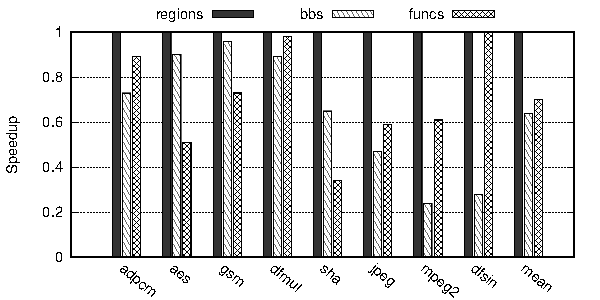
\includegraphics[width= 0.9 \linewidth]{figs/rbf_max_norm_all}
\caption{Normalized Speedup of RegionSeeker with respect to function and basic block selection, 
considering, for each benchmark, a fixed area constraint. Synthesis performed with Vivado\_HLS.}
\label{fig:regions_all}
\end{figure}

\newpage
\section{RegionSeeker MuLTiVersioning}

\HLS\ (HLS) tools, such as Vivado\_HLS by Xilinx, may employ %additional 
optimizations to HW accelerators
design in order to increase performance, i.e. obtain faster execution. These 
%pragma-directed 
HLS optimizations were not taken into account by \rseeker\ framework in the
previous section. Default, non optimized versions of HW accelerators were identified
and selected instead. In this
section we present an extended \rseeker\ framework, which performs the selection not 
only among possible CFG subgraphs, but also among different versions of each identified 
subgraph, namely different versions of the regions identified. 
We call this extension RegionSeeker: the MuLTiVersioning approach.

% The \rseeker\ framework, as detailed in the previous section, was designed in order to identify
% the most efficient HW accelerators under a given constraint, but was targeting default HW
% implementations. Pragma-directed HLS optimizations were not taken into account. In this 
% section we present an extended \rseeker\ framework, which performs the selection not 
% only among possible CFG subgraphs, but also among different versions of each identified 
% subgraph of the CFG, namely different versions of the regions identified. 
% We call this extension the RegionSeeker: MuLTiVersioning approach.

\subsection{Methodology}
\label{subsec:mv_meth}

The rationale, supporting the extension of RegionSeeker framework, is to achieve better
speedup that can be provided by exploiting a more 
varied set of HW accelerators to select from. This is being achieved by instantiating 
different versions of each HW accelerator. The parameters that were modified in order to 
design different HW implementations of the same accelerators are a) the Loop Unrolling 
(LU) factor, in accelerators that contain loops, 
b) the loop pipelining option, being either on or off, and c) the array partition factor, 
which is the number of input and output ports of the memory buffer (scratchpad) attached 
to the accelerator.\par

\subsection{Experimental Results}
\label{subsec:mv_res}

All versions of the HW accelerators were evaluated by exploiting the Aladdin HW accelerator simulator.  
Aladdin targets ASIC implementations. It
provides a fast evaluation, but does not generate a synthesizable netlist,
as opposed to Vivado\_HLS. Nonetheless, the estimations provided are
within 1\% of the ones derived from a Register-transfer level (RTL) implementation, according to 
the developers of Aladdin \cite{ShaoJul14}.
For all simulated versions of the selected regions (or HW accelerators), the number of Cycles and number 
of Functional Units (FU) Area were retrieved. For the SW execution time the gem5 simulator 
\cite{BinkertFeb11}
was used with two CPU settings: a) TimingCPU  (a simple and slow CPU with only two pipeline stages)
and b) O3CPU (a complex and fast CPU with five pipeline stages and other resources such as a 
branch predictor, reorder buffer etc). \par

The \exact\ selection algorithm, as detailed in Subsection \ref{subsec:meth}  was used subsequently to 
perform the optimal subset selection, 
given an initial set of HW accelerators along with their respective versions, as well as a specific 
area (HW resources) budget. An important note is that no more than one version of each candidate 
can be selected, as one realization of the respective SW execution is required.
Experiments were run in \jpeg\ benchmark and four different selection
approaches are presented, compared to the MuLTiVersioning approach.\par

The speedup achieved on \jpeg\ benchmark, over the respective SW 
time of the same set of selected regions (kernels) %, and the whole application 
are showcased. 
The four different approaches compared are:
a) the \emph{min} where the regions with the least amount of area are included in the set
and hence can be selected, b) the \emph{base} 
where the regions with median values of area are selected, c) the \emph{max} where only the maximum 
area regions can be selected and finally d) the MuLTiVersioning approach where any possible version 
of the regions can be selected. \par

The strength of the MuLTiVersioning approach and the benefit of having 
a variety of potential candidates to select from 
%for any equivalent computation, throughout the \jpeg\  application 
is demonstrated by the experimental outcome of the \jpeg\ application (kernels run-time). 
In Figure \ref{fig:mlv_aladdin} for any given area point, the speedup obtained is higher than any other 
methodology. For a medium area point ($200 * 10^3 uM^2$), the 
speedup achieved with MuLTiVersioning is 1.7x more than the second best, \emph{base} approach. For 
a large area constraint ($400 * 10^3 uM^2$) the MuLTiVersioning speedup is more than 2x compared to
\emph{base} and more than 6x compared to \emph{min}.\par

% In Figure \ref{fig:mlv_speed_aladdin} the same trend is depicted in the speedup of the whole application
% for the MuLTiVersioning methodology, where it constantly outperforms every other competitive method while
% reaching a maximum speedup of 1.8x over the entire jpeg application.\par

\begin{figure*}[h]
\centering
\hspace*{-1cm}
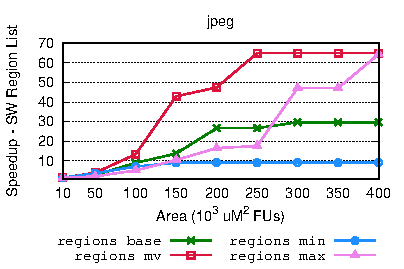
\includegraphics[width= 0.7 \linewidth]{figs/plot_O3CPU_SW_large}
\caption{Comparison of speedup obtained on jpeg benchmark, over the
SW time of the equivalent kernels (regions), varying the area constraint, using 
Aladdin and gem5 for Speedup and Area evaluation.
Four approaches are compared: The 
min where the regions with least amount of area are selected, the base
where the regions with median values of area are selected, the max where 
only the maximum area regions can be selected and finally the MuLTiVersioning
approach where any version of the regions can be selected.
}
\label{fig:mlv_aladdin}
\end{figure*}

% \begin{figure}[h]
% \centering
% \hspace*{-1cm}
% \includegraphics[width= 0.7 \linewidth]{Figs/plot_O3CPU}
% \caption{Comparison of speedup obtained on jpeg benchmark, 
% varying the area constraint, using 
% Aladdin and Gem5 for Speedup and Area evaluation.
% Four approaches are compared: The 
% min where the regions with least amount of area are selected, the base
% where the regions with median values of area are selected, the max where 
% only the maximum area regions can be selected and finally the MuLTiVersioning
% approach where any version of the regions can be selected.}
% \label{fig:mlv_speed_aladdin}
% \end{figure}


\section{Conclusions}
\label{sec:rs_conclusions}

The \rseeker\ framework, along with the \rseeker\ \multi\ extension of the former, are
methodologies that extend the \SoTA\ in the HW/SW co-design domain. They provide
efficient solutions to the problem of automatically deciding which parts of an application should
be synthesized to HW, under a given area budget. The accelerators identified by \rseeker\ 
consistently outperform the ones derived by data flow level algorithms and strictly function 
level candidates, across applications of widely different sizes and for varied area constraints.
As an example, \rseeker\ offers up to 4.5x speedup for the \mpeg\ benchmark compared to as SW
execution. This work was published in IEEE Transactions on Computer-Aided Design of Integrated 
Circuits and Systems (TCAD) journal \cite{ZacharopoulosApr19}.
The \multi\ approach extends the initial selection pool of candidates and, compared
to default HW accelerators configurations, offers enhanced speedup on the \jpeg\ application of up
to 1.7x speedup on the entire application and up to 65x speedup on the relative kernels that 
are synthesized into HW.

% \begin{figure}
% \centering
% \includegraphics[scale=0.5,angle=90]{bounded_loop_automaton}
% \caption{\textsc{Automaton} for something or other. A caption can be rather
% long and \emph{should} then consist of complete sentences ended with a `.'}
% \end{figure}

% \section{The first \textsc{Section}}

% Here is some text with \textsc{SmallCaps} in normal font.

% \lipsum[3-4]

%  \section{The second, math section}
% \begin{center}
%   \begin{tikzpicture}[shorten >=1pt,node distance=2cm,auto, initial text=, >=stealth] 
%     \node[state, initial] (q0) {$q_0$};
%     \node[state] (q1) [right of=q0] {$q_1$};
%     \node[state] (q2) [right of=q1] {$q_2$};
%     \node[state, accepting] (q3) [right of=q2] {$q_3$};
%     \path[->]
%     (q0) 
%     edge [loop above] node {0,1} ()
%     edge  node {0} (q1)
%     (q1)
%     edge  node {1} (q2)
%     (q2)
%     edge node {0} (q3)
%     (q3)
%     edge [loop above] node {0,1} ()
% ;
%   \end{tikzpicture}
% \end{center}

% \textbf{Theorem 1 (Residue Theorem).}
% Let $f$ be analytic in the region $G$ except for the isolated singularities $a_1,a_2,\ldots,a_m$. If $\gamma$ is a closed rectifiable curve in $G$ which does not pass through any of the points $a_k$ and if $\gamma\approx 0$ in $G$ then
% \[
% \frac{1}{2\pi i}\int_\gamma f = \sum_{k=1}^m n(\gamma;a_k) \text{Res}(f;a_k).
% \]
% \textbf{Theorem 2 (Maximum Modulus).}
% \emph{Let $G$ be a bounded open set in $\mathbb{C}$ and suppose that $f$ is a continuous function on $G^-$ which is analytic in $G$. Then}
% \[
% \max\{|f(z)|:z\in G^-\}=\max \{|f(z)|:z\in \partial G \}.
% \]

% \section[third]{A very very long section, titled ``The third section'', with
%   a rather  short text alternative (third)}
% \lipsum \texttt{Some Test}
% \lstset{language=algebra,linewidth=0.95\linewidth,breaklines=true,numbers=left,
% basicstyle=\ttfamily,numberstyle=\tiny,escapeinside={//*}{\^^M},
% mathescape=true}
% \begin{lstlisting}
% import IntSpec, ItemSpec;

% sort cart; //*\label{sort}

% constructors //*\label{begin-sig}
% create() $\longrightarrow$ cart;
% insert(cart, item) $\longrightarrow$ cart;
% observers
% amount(cart) $\longrightarrow$ int;
% transformers
% delete(cart, item) $\longrightarrow$ cart; //*\label{end-sig}

% axioms //*\label{begin-axioms}
% forall c: cart, i, j: item 

% amount(create()) $=$ 0; //*\label{begin-amount}
% amount(insert(c,i)) $=$ amount(c) $+$ price(i); //*\label{end-amount}
% delete(create(),i) $=$ create(); //*\label{begin-delete}
% delete(insert(c,i),j) $=$
% if (i =$\:$= j) c
% else insert(delete(c,j),i); //*\label{end-axioms}
% end
% \end{lstlisting}

% As you can easily see from the above listing \citet{bbggs:iet07}
% define something weird based on the BPEL specification
% \citep{bpelspec}.
% \nocite{*}

% \appendix %optional, use only if you have an appendix
% I removed mine a year ago.

\chapter{Optimizations applied to HW Accelerators}

\section{Data reuse Analysis}


\subsection{Motivation}
Loops are ideal candidates for acceleration. In almost every application, there is a
number of them that contain a large number of iterations and there is a sufficient 
amount of computation taking place in their bodies. In addition to that, there are 
nested loops which commonly show a high level of data reuse. An example of such high
data reuse can be observed in sliding window applications, where there is typically
a window of accesses scanning a wider domain, such as a two-dimensional array. 
Given that the level and pattern of data reuse is known a priori, it would be feasible 
to design specific memory structures, also known as memory buffers, attached to the 
HW accelerators. These memory buffers can exploit data reuse by keeping data locally 
and, hence, minimize the memory latency due to communication with the main memory.\par
 %while exploiting the computational potential of the accelerators.\par
\subsection{Related Work}

In the domain of identifying automatically accelerators, research has 
so far focused mostly on accelerating data-flow~\cite{GiaquintaMar15} \cite{GutinFeb12}, 
not taking into equal account the potential for optimization by memory accesses. 
Exceptions are provided by papers \cite{BiswasMar06} \cite{ HaaBOct2014}
where the authors support the claim that accelerators with custom
storage can provide better speedup compared to the ones that
accelerate data-flow only. However, these papers focus on the
identification of the accelerators, and do not present a methodology 
to automatically identify the optimization potential, as well as
synthesize them accordingly.\par
In sliding window applications, there are research endeavors
both by academia and industry to exploit data reuse. The smart
buffers~\cite{GuoJun04} generated by the ROCCC
compiler~\cite{VillarrealMay10} allow for automatic detection of data
reuse opportunities, but cannot be interfaced 
with interconnects of varying width.
The commercial Vivado\_HLS tool requires
extensive manual rewrite of the source code, in order to instantiate
a reuse memory buffer. On the other hand, the approach presented 
% in \ref{sec:2_1_meth} 
here relies on automated code
analysis to derive the characteristics of the target application.\par 

\section{Machine Learning Approach for Loop Unrolling Prediction}


\chapter[System Aware Accelerators Identification]
{System Aware Accelerators Identification --- Speedup gain and Energy Saving}
%--- \\AccelSeeker and EnergySeeker}

\section{\aseeker}

\section{EnergySeeker}

\chapter*{Conclusions}
\addcontentsline{toc}{chapter}{Conclusions}


\backmatter

% \chapter{Glossary} %optional

%\bibliographystyle{alpha}
\bibliographystyle{abbrv}
%\bibliographystyle{dcu}
%\bibliographystyle{plainnat}
\bibliography{biblio}

%\bibliographystyle{abbrv}
%note that all bibliography is now in cvs in ../bibl/bibl.bib hence the line below
%\bibliography{/Users/GiorgioZacharo/bibl/bibl}
%
% \cleardoublepage
% \theindex %optional, use only if you have an index, must use
% 	  %\makeindex in the preamble
% \lipsum

\end{document}
